\documentclass[conference,a4paper]{IEEEtran}
\usepackage[pdftex]{graphicx}
\usepackage{url}
\usepackage{grffile}
\usepackage{eurosym}

%\usepackage[pdftex]{hyperref}
%\hypersetup{%
%pdfpagemode=UseNone,%
%a4paper,%
%pdffitwindow=true,%
%colorlinks=true,%
%linkcolor=black,%
%citecolor=black,%
%urlcolor=black,%
%filecolor=black,%
%pdftitle={Smart Phone Interfaces to Wireless Health Sensors},%
%pdfauthor={Hugh O'Brien, Pepijn van de Ven, John Nelson, Alan Bourke},%
%pdfproducer={LaTeX}
%bookmarks=false
%}

\begin{document}

\title{Smart Phone Interfaces to Wireless Health Sensors}
\author{Hugh~O'Brien, Pepijn~van~de~Ven, John~Nelson, Alan~Bourke,
\\
Department of Electronic and Computer Engineering,
\\
University of Limerick, Ireland}

\maketitle

\begin{abstract}
This paper discusses user and system interfaces for mobile health-monitoring systems.
Current approaches often use entirely web based solutions, however with mobile phones
being extremely widespread and becoming ever more powerful, there is
a strong case to be made for their use as interfaces to wearable health sensors. Phones provide a socially appropriate means of displaying timely information to the
user and enable the sensors to transmit measurements directly to health care providers.
In this paper we demonstrate the advantages of their use in this manner; outline the current consumer smart phone landscape from this perspective and introduce an information architecture for sensor message management on mobile devices. The
architecture focuses on ease of access to constantly updating sensor readings and allows many data sources to feed many data consumers simultaneously. While designed for use with a fall and mobility sensor, it may be equally well adapted for use with any other
health or vital signs sensor. 
\end{abstract}

%\begin{IEEEkeywords}
%wireless sensors, user interfaces, smart phones, digital health
%\end{IEEEkeywords}

\section{Introduction}
With the world's population greying at an alarming rate,
%UN Population division tables reference?
many countries are experiencing increasing pressure on their health care infrastructure. These systems have traditionally relied on in-hospital treatment of patients, and the detection of potential ailments is normally the role of the general practitioners. However, due to infrequent patient visits, possibly due to the disabling effects of an illness, this approach is far from infallible. Mobile health monitoring systems stand poised to fill this information deficit and will have an important role to play in the near future; both in improving the likelihood of detecting ailments at an early stage, when the need for in-hospital treatment can be averted, as well as to easing the increasing strain on health care infrastructures. It is for these reasons that the European Community is supporting a large number of research projects including the recently successfully finalised CAALYX project \cite{BourkeCan1} (continued in the eCAALYX project), the MyHeart intelligent clothing for cardio-vascular treatment project and the Wealthy wearable health care system.

The detection of falls is of particular importance among mobile health monitoring systems targeted towards the elderly. Falls are a substantial threat to elderly citizens and on average, are experienced by one in three people over the age of 65 at least once a year. The resulting emotional and financial cost to individuals and society is significant. In a recently published paper \cite{Gannon2008}, Gannon et al. estimated the annual cost of falls amongst Irish elderly citizens to be \euro 404 million. In the United States the cost of falls for people aged 65 and over was estimated at over \$19 billion during the year 2000 \cite{Stevens2006}. People who suffer from reduced mobility, in particular the elderly, can benefit greatly from having a fall and mobility sensor for several reasons.
%REFERENCE?
In the event of a fall, it is of prime importance that help is requested immediately to prevent a `long-lie' event \cite{WildBMJ}. All too often, victims of a fall spend hours or longer suffering on their own before being discovered. Receiving immediate medical attention has shown to lower the risk of hospitalisation by 26\%, and death as a result of the fall by 80\% \cite{Noury2008}. To prevent falls from occurring in the first place, it is important that elderly people (or other groups of citizens at higher risk of falling) and their health providers have access to an early warning system that indicates when the patient's condition may lead to an increased risk of falling. Mobility monitoring is a proven means of measuring fall risk
%REFERENCE???
and a continuous assessment of an elderly person's mobility is therefore very valuable. Most commercially available systems rely on a base station in the patient's home to report incidents to care staff, but a portable fall monitor would grant the same level of care to the patient while they are outside. 

Modern mobile phones possess a dizzying array of features and technology; they are mass produced to keep per unit costs low and have gained complete acceptance into the lives of most in the industrialised world.
Many devices feature processor and memory capabilities comparable to desktop computers of yesteryear; and while it has been historically difficult to access their capabilities, successive generations have exposed more and more functionality to third-party development.

Their long range, high speed communication abilities combined with personal area network radios make them technically appropriate targets, while their pervasiveness, and the level of acceptance they have gained in the consumer's mindset accords them the enviable position of being \textit{socially} appropriate targets.
We therefore propose that a strong case exists for their involvement in the rapidly evolving health data market; they are capable of providing the missing link between sensor readings and changes in user behaviour.

In this paper, section \ref{CurrentMeth.sec} presents the advantages mobile phones can offer to health monitoring systems. The communication channels presently available for development are discussed in section \ref{Communication.sec}. After a concise overview of available mobile platforms in section \ref{MobPlatforms.sec}, a detailed case study targeting the aforementioned fall detection is discussed in section \ref{Interface.sec}. 


\section{Advantages of Mobile\label{CurrentMeth.sec}}

\begin{figure}[t]
\centering
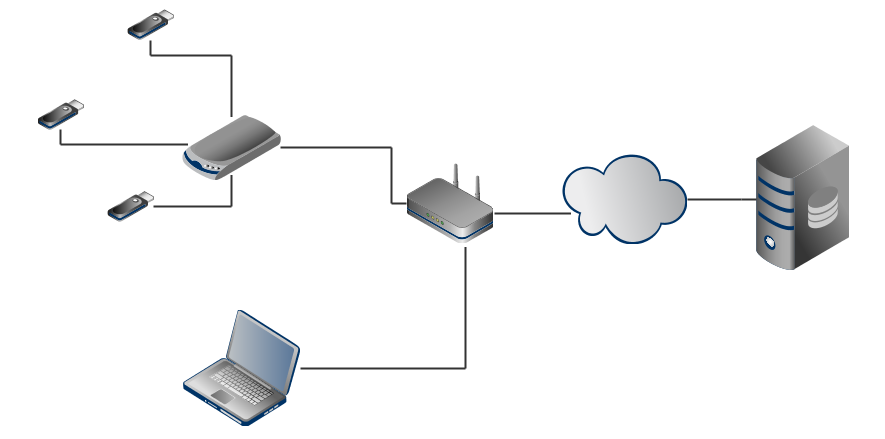
\includegraphics[scale=0.27]{./figures/currentFlow.png}
\caption{Typical data flow in current systems. To the left, wireless sensors communicate with a sensor base station. This station accesses the user's Internet modem to send the sensor readings to a remote server. To view these readings, the user connects to the server using their personal computer.}
\label{figCurFlow}
\end{figure}

Current health monitoring systems often rely on the use of a base station or hub in the home environment. In order to process the data that sensors generate, the hub transmits the readings to a remote server for storage and analysis.
This data flow is shown in Figure \ref{figCurFlow}.
A hub device specific to the particular sensor provider typically acts as a mediator between the low powered radio communication from the sensors and the patient's home broadband connection.
To review the data, users such as the GP, caregivers and the patients themselves, connect to the provider's service, via their browser, and access the records in a graphical form. This method presents a number of drawbacks:

\begin{itemize}
\item The hub device must be provided with a constant Internet connection through which to send updates.
Many remote areas do not possess the infrastructure to support these types of connections; precluding such users from participating.
\item
The user's access to their data is dependant on their access to the Internet and the reliability of the provider's central storage system.
Should the user simply not wish to purchase an Internet connection they would be unable to access their data, despite it being generated within their own home.
More worryingly, the longevity of the user's data is contingent on the survival of the provider's business, many of which are recent start-ups.
\item
The user's data is disclosed to a third party. As the service is provided over the Internet, the provider may potentially be located in another country and not be subject to the privacy regulations the user is accustomed to.
This issue is most apparent when medical data is considered, as even in a home scenario, the user may not wish their information to be visible to other users of the same computer.
Comparatively, mobile phones are devices which are rarely shared.
\end{itemize}


\begin{figure}
\centering
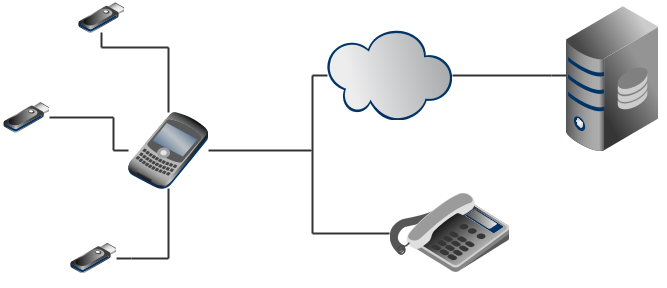
\includegraphics[scale=0.27]{./figures/propFlow.png}
\caption{Proposed method with direct human contact. Wireless sensors communicate directly with a smart phone. The user may directly access the data and the phone may forward the readings to a remote server. Should a reading require immediate attention, the phone may make direct contact with the patient or a care giver. Note that the system is now portable.}
\label{figPropFlow}
\end{figure}

Phones possess considerably better connectivity options than most desktop computers; 3G/GPRS data connections are standard and offer network access in remote locations. Bluetooth allows low power data connections within the home without incurring carrier fees, and most compellingly, smart phones have direct access to the telephone network, granting their software the ability to directly contact, on-demand, any person that may need immediate notification of specific sensor events.

Indeed, this capability is perhaps the most attractive benefit of using mobile devices.
In medical situations, where the owner of the phone may be the subject of the sensor readings, alerting the phone owner to a critical medical event would serve little purpose, immediate notification of a third party is required.
The vast majority of modern data communications revolve around systems contacting other systems. In most cases, the closest a system can come to direct human contact is an email, which still requires the receiver to check their inbox, perhaps some time after the mail was sent.
By crossing into the public switched telephone network, typically reserved for human to human interaction, a phone based alert system gains a direct line to a human contact, while simultaneously bypassing the many potential failure points of the average data network.
The time benefit this accords is crucial as any delay in receiving care places the patient at increased risk. Such a data flow is illustrated in Figure \ref{figPropFlow}.

During regular operation, sensor data is available to the phone and may be viewed by the user as it is produced, in a manner as easily accessible as the viewing  of an SMS message. Phones provide a direct line of communication from the system to the user with a timeliness that PC browser based systems cannot match. Events or alerts detected by the phone or the remote server can be immediately presented to the user in an automated fashion. Considering the cases of drug adherence or over-exertion during physical rehabilitation, it is clear how such patient-centric alerts would be advantageous.

Modern phones are capable of storing gigabytes of data on removable memory cards, allowing them to take on the role of data storage with little impediment to their normal functions.
Should the data be stored in a standardised format then various third party software applications may be developed that analyse the data in novel ways.\footnote{Potentially creating a market for health analytics.}

Finally, as mobile devices are necessarily equipped with high capacity batteries, the potential exists for users to recharge their sensors from the phone, which would provide a more sustainable form of power than simply replacing cells or discarding the sensor entirely.
Higher power sensors such as those encountered in medical scenarios\footnote{Pulse Oximeters, for example, consume considerable energy in powering LEDs bright enough to be visible through a human finger.} could also be accommodated by such a system.

\section{Sensor Communications\label{Communication.sec}}
This section gives a brief overview of the communication facilities available to smart phones and to most sensors. At the time of writing, Bluetooth is the only technology that significantly overlaps both classes of device.

\subsection{IEEE 802.15.4}
IEEE 802.15.4 defines low powered, short range, best effort wireless networks that operate in the 2.4GHz ISM band.
The standard limits itself to describing the physical and media access control layers; leaving further definitions up to higher level implementations such as ZigBee\footnote{Other implementations include `WirelessHART' and `MiWi'}.
802.15.4 has a nominal range of approximately 10 metres and a maximum transfer rate of 250Kbps, power consumption is typically in the region of 20mA.
The low power nature of this technology has made it the de-facto standard amongst distributed sensor networks; were it available on mobile devices it is likely that phones would already play a large role in sensor interaction; however it is unlikely to find its way into handsets in the near future, as, for the time being, little manufacturer incentive exists to do so.

\subsection{Bluetooth}
Bluetooth is a mature, open wireless protocol also operating in the 2.4GHz band that is designed for medium data rate, best effort communications over a relatively short distances; it has an average data rate of approximately 2Mbps and a typical range of between 10m and 50m.
Bluetooth implements various forms of error correction chosen automatically based on the detected channel properties; encryption is also specified.

Bluetooth is a well accepted consumer technology with many users utilising it for file transfers between phones or to connect with wireless headsets. Due to the dwindling costs of fully integrated Bluetooth chipsets it is now uncommon to find a modern handset that does not support it.

Low cost Bluetooth modules are widely available but are an uncommon sight on sensor motes, the notable exceptions being the SHIMMER and the Mulle.
The protocol is seen as too power expensive for typical sensor applications; furthermore, it suffers from long connection setup times, an unwelcome feature for low power sensor networks, though less of an issue in the context of personal medical sensors.

\subsection{Bluetooth Low Energy Technology}
Bluetooth low energy addresses the power concerns associated with standard Bluetooth while retaining compatibility with the many existing Bluetooth devices.
This low energy extension to the Bluetooth standard inherits the open licensing of its parent technology but reduces the throughput roughly to the same level as 802.15.4.
The time required to transmit a data packet has been greatly reduced, ensuring that the radio is powered for as little time as possible.
Peak current draw is limited to 15mA, enabling the radio to be powered from a coin cell battery.
Existing handsets should be able to fully access sensors equipped with low energy radios once they have received a software update.

\subsection{Wi-Fi}
IEEE 802.11 wireless LAN chips are found in the majority of recent smart phones.
Wi-Fi is a high power, high data rate protocol that uses relatively expensive hardware.
It is not suitable as an interface to wireless sensors, however it should not be overlooked as a connectivity option should the handset wish to transfer a large quantity of data to a remote server at one time.

\section{Platforms for Mobile Development\label{MobPlatforms.sec}}
There are a great many mobile platforms available, each at varying stages of maturity. An outline of several currently dominant platforms is given below, with a focus on their suitability as sensor gateways.

\subsection{Java Micro Edition}
While most mobile operating systems are directly tied to specific manufacturers or even to specific models, `Java 2 Micro Edition' commonly referred to as J2ME offers a subset of the Java platform that provides a collection of APIs common across all devices that implement the standard.
These APIs were chosen to aid in the development of applications for devices constrained by processing power as well as by small displays and lack of mouse or keyboard. 
J2ME was, and remains, widely implemented on almost all commodity mobile devices of the last five years, however it is noticeably absent on several recent high profile smart phones.
APIs exist for byte level access to Bluetooth connections, Internet access, as well as persistent storage on the device.
As J2ME applications are constrained within the Java virtual machine they are often unable to access features of the device considered `sensitive'.
Such features often include telephony functionality which may limit the full utilisation of the device.
However even with these restrictions it still represents by far the greatest installed base and provides full Bluetooth support.

\subsection{Android}
Android is a mobile operating system developed primarily by Google, it is based upon the Linux kernel and is available under an open-source license.
Several handset manufacturers have released products based on the technology.
Android applications are written in Java, however unlike the J2ME where Java applications are less privileged than native applications, Android Java applications form the base of the entire operating system and are able to make use of the majority of the device's functionality.
After some delay, full Bluetooth support has been recently implemented. Due to a non-standard virtual machine, J2ME is not supported.

\subsection{Symbian}
Most commonly encountered on Nokia `business' phones Symbian offers the developer complete access to the device.
Symbian programs are written in C++ which poses some issues for portability, however most phones will also provide a full J2ME virtual machine.

\subsection{iPhone}
The iPhone imposes considerable restrictions on developer access to the device's hardware functionality. Bluetooth support is intentionally limited.

\subsection{BlackBerry}
Akin to Android, BlackBerry devices are entirely Java based and as such combine the best features of J2ME with a rich set of extra APIs.
There is a wide variety of connectivity options and Bluetooth is fully supported.
In addition, large parts of the underlying operating system are exposed to developers allowing for detailed customisation and integration.


\section{information architecture for sensor data\label{Interface.sec}}
To further explore the advantages of using mobile phones as the primary interface to health sensor motes, the authors are currently performing studies with an in-house built, fall and mobility sensor which communicates with a Blackberry handset. The fall and mobility sensor consists of a Texas Instruments MSP430 micro-controller, Freescale 3-axis accelerometer and a Roving Networks Bluetooth module \cite{VandeVen2009}. The algorithms used in the fall and mobility sensor have previously been discussed in \cite{BourkeCan1} and \cite{BourkeCan2}.

In addition to the evident importance of reliable fall detection capabilities and the prompt relay of related messages to a caretaker or rescue services, an important aspect of fall and mobility monitoring is the feedback that such devices can give to the user.
In many cases, the most effective means of preventing or overcoming mobility issues is frequent and sufficient exercise.
The fall and mobility monitor can aid the user in complying with a set treatment programme by monitoring the user and suggesting further exercises to meet targets.
This application clearly demonstrates one of the main benefits of using a mobile phone to interface with the sensors; the user is immediately provided with feedback which can improve treatment, and this information is presented on a device that most, if not all, user groups are familiar with\footnote{Phones with large touch displays are currently becoming increasingly popular. These phones offer accessible interfaces for less technologically experienced users or users with reduced motor skills}.
Caretakers and health professionals can access the data extracted from the users mobility patterns through any of the transport mechanisms the phone provides.

This section details the architecture used on a BlackBerry `Storm' device acting as interface to the sensor. A modular system has been a key design goal, as has attempting to keep the code base small and efficient for use on resource constrained devices such as phones (it is unrealistic to presume that the sensor application will be the only application in use on the device).

In practice, the application appears alongside other applications on the device, though it is automatically started at boot time. When started it reconnects to the most recently connected fall sensor and begins processing and logging data. There are options to activate or deactivate various agents that act on the data, and once running the application may continue to function in the background as the phone is used for other purposes. If a fall is detected, the user is prompted to cancel the alert. If not cancelled within a short period of time the phone dials a preset number. Non-urgent data such as step counts are processed in the background, with the user being alerted if they have missed or exceeded any thresholds prescribed to them. Raw sensor data may be logged to the device's internal memory for debugging, and the results of basic on-device processing may be sent to a remote server for further logging and analysis. Though not currently implemented, the potential exists for the application to estimate the user's location if such information is deemed necessary.

%The top level of the design consists of graphical user interfaces and agents. The concept and function of agents will be further discussed after a discussion of the low level layers in the architecture.

\subsection{General Overview}

Please refer to Figure \ref{figArch} for a visual representation of the architecture. The Bluetooth connection from the sensor is visible as a stream of bytes on the BlackBerry handset. A message protocol was defined with a fixed header size and specific start and stop bytes. For each sensor connection on the handset a state machine monitors the byte stream to detect when a valid message has been seen. The checksum of the message is computed, and if valid, a new SensorMessage object is created by the state machine. The state machine then resets its state and is ready to begin watching for the next message. 

The SensorMessage object creates a SensorHeader object, which accesses the raw bytes stored in the SensorMessage and parses them into native data types. The SensorHeader also logs status information to the DataStore.

Using the message type information gleamed from the SensorHeader, the SensorMessage dispatches the remaining raw bytes to the appropriate message handler defined for the particular message type received. e.g. a mobility message contains information on the user's cadence so a MobilityMessage object parses the bytes according to the defined structure of a mobility message and stores the extracted values in the DataStore.

The DataStore acts as the division between the lower and the higher layers of the interface. The lower layers are unconcerned with how or whether the information they provide is used, they need only forward their readings. All records stored in the DataStore are interactive objects, which maintain their own value and a list of Agents who require notification when the value changes. Agents may register for updates on records that do not yet exist, so that if the record should ever receive data from the lower layer, the agent will be immediately informed.

Agents monitor records, such as `step count', and may either present this data to the user in the form of a graphical screen (as in figure \ref{MobilityInterface.fig}), store the data in the device's flash memory, upload the data to a remote server, or in the case of an emergency, make use of the handset's telephony features to directly contact emergency services.

\subsection{ByteSources}

At the bottom of the stack are the ByteSources. The function of this layer is to abstract the source of the data, be it the Bluetooth radio, simulated data, or otherwise, such that the ByteSources may buffer data as it is received and push the individual bytes of the data one at a time into the next layer, the MessageVerifier. Each ByteSource is required to create its own instantiation of a MessageVerifier (described below). For reasons relating to the functionality of upper layers each ByteSource also passes its object (a.k.a.`this') reference into the constructor of its personal MessageVerifier.

\subsection{MessageVerifier}
The MessageVerifier class models a state machine that is responsible for ensuring that the bytes passed into it from a ByteSource match an expected sequence and conform to the defined message protocol. Internally, bytes are input in a piecemeal fashion strictly from a single ByteSource and are stored in memory that is managed by the MessageVerifier. The internal state machine monitors the number and contents of the received bytes and when it has determined that enough bytes have been received that they constitute a message, it performs a simple XOR checksum. Should the message pass all of the tests, the MessageVerifier creates a new instance of a SensorMessage passing it the raw valid message as well as a reference to the ByteSource that created the message. 
The MessageVerifier does not hold a reference to this new SensorMessage and once it has been created the state machine will reset and be ready to begin processing the next message.

\subsection{SensorHeader}
Though the MessageVerifier passes a valid message into a SensorMessage constructor, the very first action of the SensorMessage constructor is to pass the same valid message into a new SensorHeader, for this reason it will be described first. The SensorHeader is processed much like any of the other messages, the key difference being that header data is always present regardless of the message type being received. 

Three features differentiate it from the other message handlers, firstly it is responsible for comparing the sequence number of the message against the expected sequence number. If these numbers do not match, an error is logged in the DataStore. If they do match then the next expected sequence number is updated.

Secondly, the SensorHeader is capable of logging detailed statistics on the frequency of messages of differing lengths and types. This is controlled through a toggle value in the DataStore. 

Thirdly, the SensorHeader parses and makes available key message values such as the type of the received message and the identification number of the sensor that provided it. This allows other message handlers to concern themselves solely with the content of their specific message type, while providing a common means of accessing the header data. The message type value in particular is required by a SensorMessage and is the reason the SensorHeader is created first.

\subsection{SensorMessage}
As described above, a SensorMessage will first create a SensorHeader for the message it received. With the parsed header the SensorMessage can determine which of the message handlers to pass the unprocessed message payload to. It is possible the system will be passed a message type it is not familiar with as new sensors are developed, for this reason logging and error handling also take place here.

\subsection{SensorRecords}
SensorRecords represent the fundamental data storage unit within the DataStore. At a basic level, a SensorRecord may be viewed as a wrapper for a single integer value. The defining feature of a SensorRecord is that it maintains a list of objects that implement the Observer interface and provides methods for additional Observer-implementing objects to be appended to this list. Classes that implement Observer provide a publicly accessible method called \verb#update()# that takes an Observable object as a parameter. SensorRecord extends the Observable class such that when a SensorRecord receives a new integer value to store (handled by the DataStore), should it decide that the value is different enough to warrant notifying the objects that are observing it, it will iterate over its list of Observers calling the \verb#update()# method on each of the elements, passing itself as the only argument. The Observers can use the accessor methods defined in SensorRecord on the Observable object reference they receive to find out exactly which SensorRecord it was that triggered the update. This is necessary as the same Observer may be observing a multitude of Observable objects yet each of them, after receiving new data from the lower layers, will call the same \verb#update()# method on the Observer.

\subsection{The DataStore}
The DataStore provides access to SensorRecords. It contains only static members and methods, it is always available and no other part of the system is responsible for instantiating it. At its heart is a hash table with Strings as keys and SensorRecords as entries. 
When queried, DataStore will first scan the hash table to determine if the record being queried already exists. Instead of returning an error in the case of a non-existent record, DataStore will automatically create the record with the default value of zero and will carry out the rest of the request on the newly created record as normal, e.g. if the store method was called it will change the value in the new SensorRecord from zero, to the specified value. The reasoning for this behaviour is to reduce the coupling between agents and SensorRecords. Should an agent attempt to observe a SensorRecord that had not yet been created because the message type that creates it has yet to be received then there would be no clear mechanism for the agent to be notified should the record be created later in the session. By registering on an empty record the agent is able to ensure that should this record ever receive an update, it will be alerted through its \verb#update()# method.

\subsection{ConfigDB}
Storing observable records that represent the current state of a sensor has immediate usefulness, but the limitation on what data can be stored (integers only) has made it difficult to use the DataStore to store anything else, such as the list of currently connected sensors or the set of user defined options that control the interface itself. For this reason a separate DataStore was created which does not have the requirement to return SensorRecords when queried. The ConfigDB does not allow new entries to be created dynamically as the regular DataStore does, if an attempt is made to access a record that does not exist then an exception is thrown.

\subsection{SourceList}
The SourceList stores the list of all sensor source IDs that have been seen by the system along with a reference to the ByteSource that was responsible for them. In SensorMessage, after the header processing but before the dispatch to the message handlers, the source ID of the message is sent to the SourceList. The SourceList is designed for agents that monitor records and may find it necessary to transmit data back to the sensor that generated the record. Normally agents are concerned only with the value of a sensor reading, not its origin, but with the SourceList an agent may acquire a reference to the ByteSource from which the message originated and call the \verb#sendToSensor# method on it. This is currently used for the delivery of acknowledgement messages to the fall sensor.

As SourceList extends the Observable class, agents may register as Observers of it so that they are notified when a new sensor becomes connected to the phone. In this way an agent may immediately begin observing records of interest that the new sensor may have generated. 

\subsection{Agents}
Agents are applications that interact with the contents of the DataStore, and, based on what they find or determine through calculation, will initiate some action or write some value back to the DataStore. Agents are self-contained and conduct all of their communication through the DataStore (i.e. an agent may observe the output record of another agent). Many agents may be `running' simultaneously and each may observe any number of SensorRecords or other observable objects. Agents represent the top layer of the component stack and offer a flexible way to expand the functionality of the interface. All agents extend the `Agent' class which exposes start and stop control to other aspects of the system. 

An example of an agent for the fall sensor interface is the FallHandler agent which monitors the \verb#status.falldetected# record on a number of different sensors and uses the BlackBerry OS integration features to place a phone call to a user-changeable telephone number (stored in the ConfigDB). A further example is the \hyphenation{Fall-Alert-Acknowledger} FallAlertAcknowledger which implements a protocol requirement that the sensor receive an acknowledgement message after alerting the phone to a fall event. Both agents also observe the SourceList and register themselves on the appropriate records anytime a new sensor becomes connected to the interface.

Agents may also be used to log data to external media, to interact with a web service, to compute user mobility patterns based on sensor data, or implement virtually any other high-level functionality. The strength of the agent based approach is demonstrated by the potential for an agent to reprogram a sensor with a new version of its firmware should one become available. This could for example be done by the web service agent, who may download the firmware to the device and signal the reprogramming agent which may or may not run as determined by user preferences.

Another useful agent is the high level `agent manager' which reads the ConfigDB to determine which agents to start at boot time or when the application is launched (e.g. the GUI agent would not be started at boot time). There is also a `connection manager' agent that ensures the sensors are continuously connected and alerts the user if a connection issue exists.

\subsection{Graphical Interfaces}
Graphical interfaces are implemented as a special form of agent. Their main goal is to access the DataStore and represent the information found there in a visual manner to the user. As they may observe any record, the graphical interface dynamically updates anytime new information is received from the sensor. User modifiable preferences are also exposed through a graphical agent.

\section{Trial Results}
The system has successfully been used in technical trials with a new type of fall sensor built in the University of Limerick. In these trials the emphasis was on the direct feedback of mobility information to the user. In addition, upon detection of a fall, agents were used to call a pre-programmed number without any user interaction. Figure \ref{MobilityInterface.fig} shows the current activity the user was performing and the number of steps (cumulative per day) and cadence (average number of steps per minute).

Trials with elderly users are planned to investigate the effect of direct motivational feedback and exercise suggestions. To this end five elderly people will be equipped with a Bluetooth enabled fall and mobility sensor and a Blackberry Storm handset. The handset will provide continuous feedback to the user and will keep track of daily activity levels. Based on targets set by the user's general practitioner, the interface will suggest exercises and give motivational messages to the user. Any changes in the activity and mobility of the elderly users will be tracked and recorded to investigate whether the direct feedback provides a stimulus for the elder to pursue appropriate levels of activity.

\begin{figure}
\centering
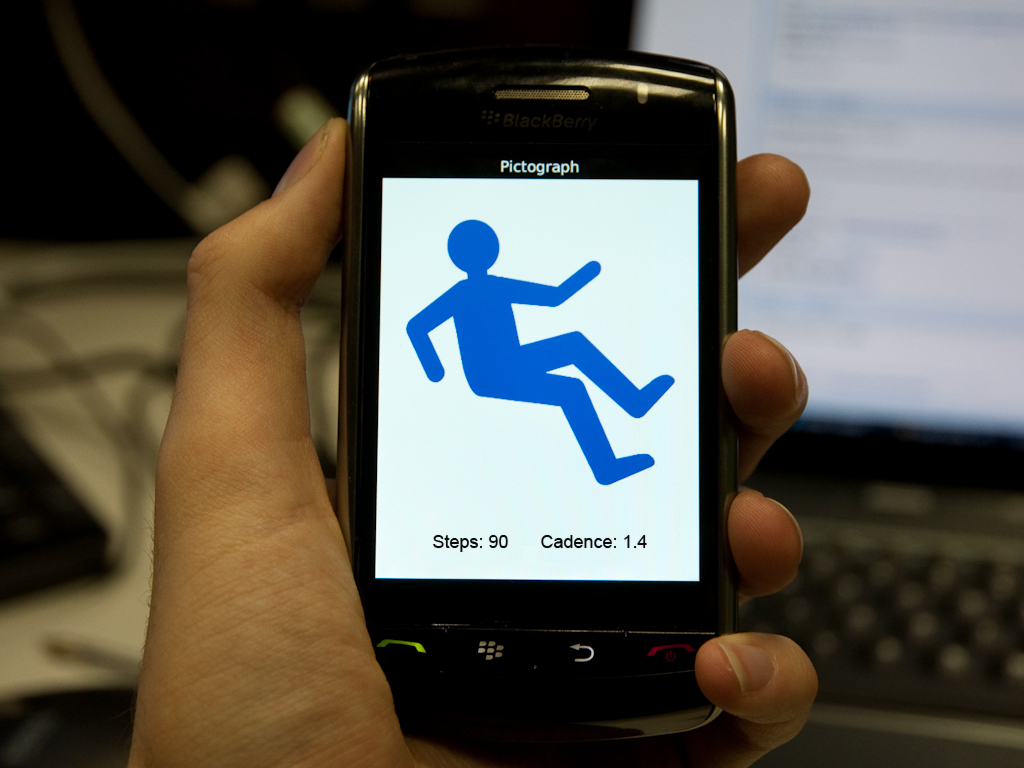
\includegraphics[scale=0.245]{./figures/storm-mod.png}
\caption{Pictorial representation of the user's state when a fall has been detected. Also shown are step count and cadence information.}
\label{MobilityInterface.fig}
\end{figure}

\section{Conclusions\label{Conclusions.sec}}
This paper has illustrated the advantages of using mobile phones both as communication links and as patient interfaces, in mobile health monitoring systems. To demonstrate the feasibility of such a system, an architecture that was implemented on the Blackberry platform was described. This architecture was used to handle messages originating from a fall and mobility sensor, but the architecture has been designed in such a way, that it may be easily used with any other type of sensor, or indeed multitude of sensors. The system has been tested in technical trials and trials with elderly people will follow, to obtain information on how the patient's activity can be influenced through direct mobility feedback.

\section*{Acknowledgement}
The authors wish to extend their gratitude to Research In Motion for their generous support.

\begin{figure}[t]
\centering
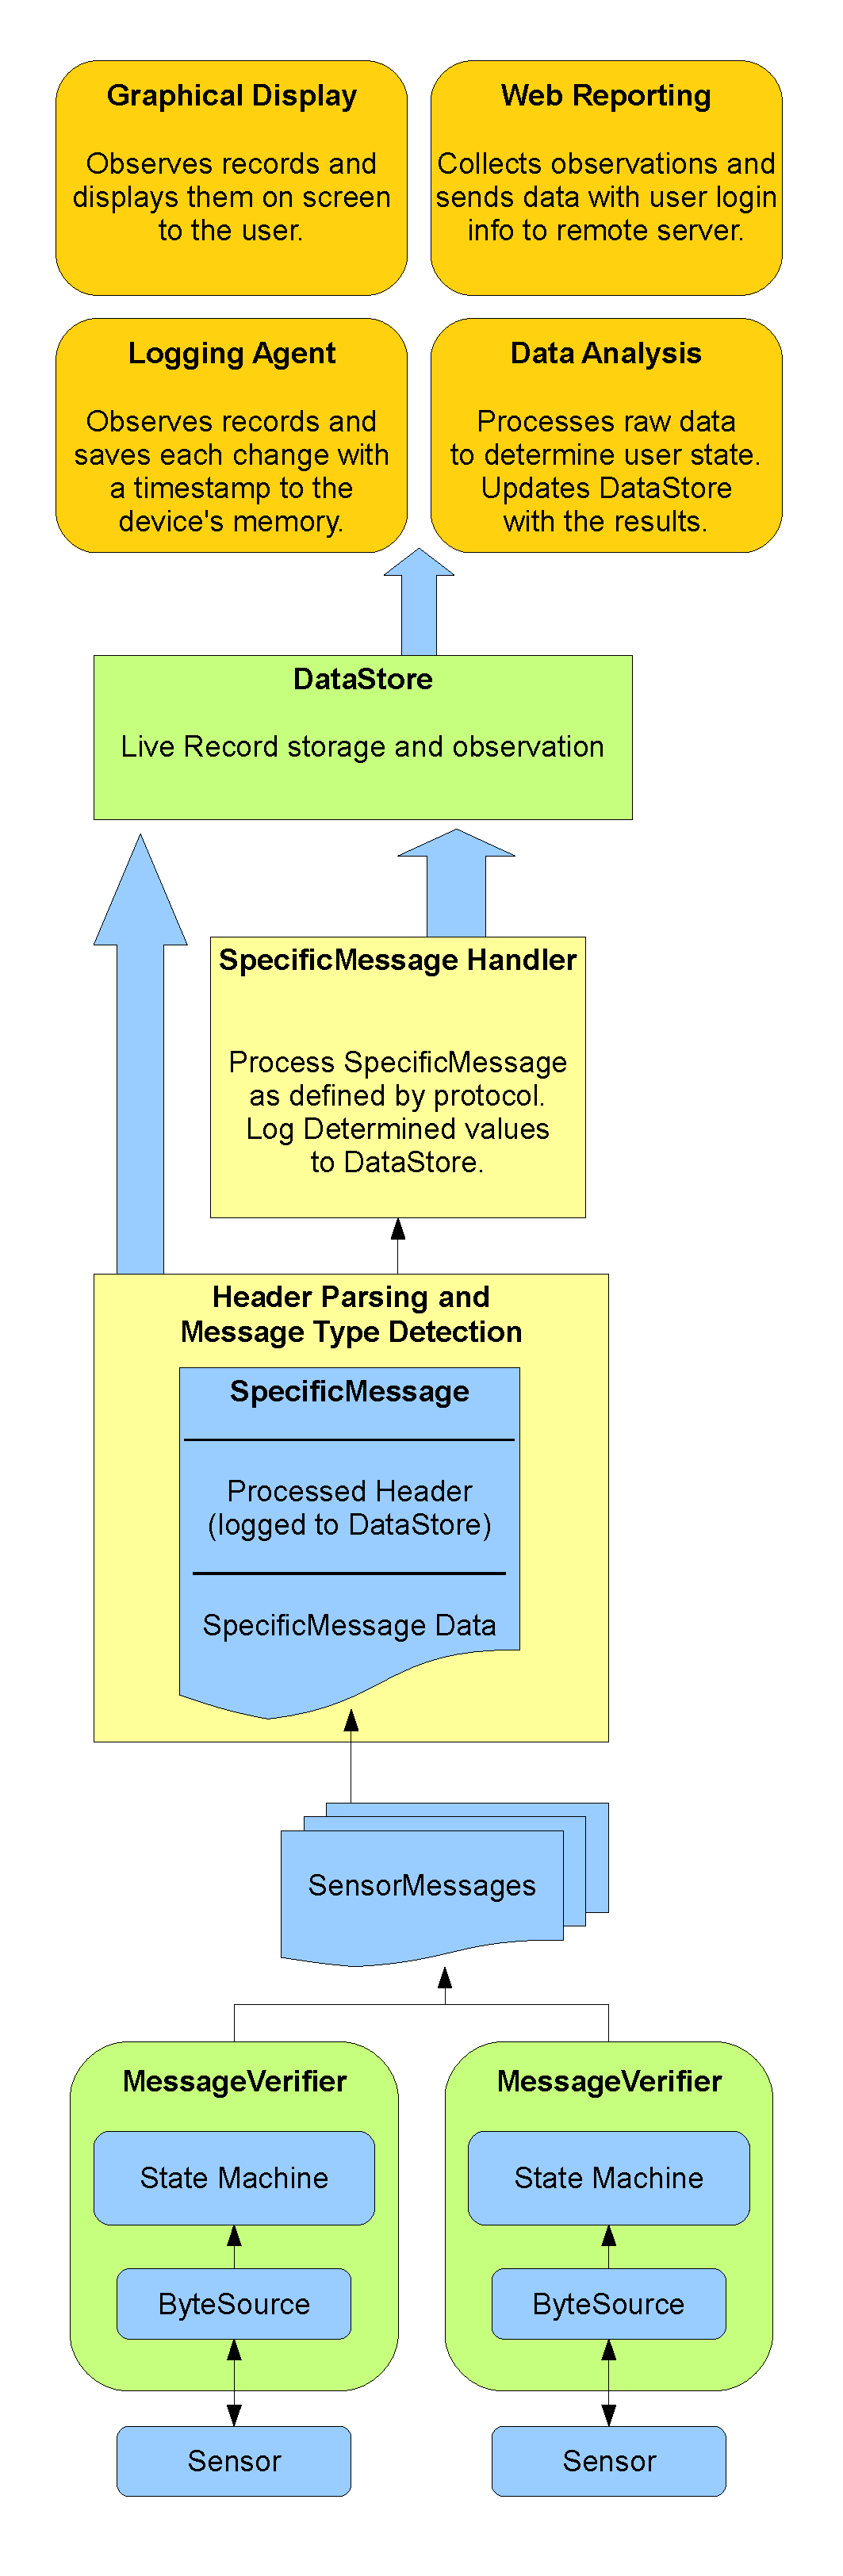
\includegraphics[scale=0.355]{./figures/column.pdf}
\caption{Visual representation of the layering model.}
\label{figArch}
\end{figure}


\bibliographystyle{IEEEtran}
\bibliography{IEEEabrv,Postdoc}


\end{document}
